\section{结果与分析}
\subsection{实验设置与评价指标}
目标高度600\,km，初始质量60000\,kg、干质量1200\,kg、有效排气速度4500\,m/s。地球半径6371\,km、引力参数$3.986004418\times10^{14}$\,m$^3$/s$^2$；$\rho_0=\rho_{\rm ref}=1.225$\,kg/m$^3$、$H_a=8500$\,m、$C_D=0.35$、$A_f=2$\,m$^2$，两向参考扰动标准差均为0.1\,m/s$^2$。实验依次评价三种规划器的收敛与终端求解性能、搜索结果的数值敏感性，以及纯PSO参考在新扰动下的开闭环执行精度。

\subsection{无精修规划器对比}
本组实验比较三种算法在相同计算预算下获得可行入轨轨迹的能力。每种算法执行五次配对运行，每次使用17376次搜索评价，最终两次独立ODE复核作为统一的额外验收开销。表\ref{tab:algorithm}汇总高精度复核统计，图\ref{fig:algorithm}给出随评价次数变化的搜索目标中位数、四分位区间及全部最终复核值。
\begin{table}[htbp]\centering\small
\caption{等预算无精修比较（每种算法五次）。IQR为25\%--75\%区间，耗时不含编译与复核。}\label{tab:algorithm}
\begin{tabular}{lcccc}\toprule
算法 & 复核目标中位数 & IQR & 通过数 & 耗时中位数/s\\\midrule
PSO & \ensuremath{1.75\times10^{-6}} & [\ensuremath{1.22\times10^{-6}}, \ensuremath{2.32\times10^{-6}}] & 5/5 & 3.24\\
GA & \ensuremath{2.29\times10^{-4}} & [\ensuremath{1.90\times10^{-4}}, \ensuremath{5.49\times10^{-4}}] & 0/5 & 3.24\\
SA & \ensuremath{5.22\times10^{-3}} & [\ensuremath{2.70\times10^{-4}}, \ensuremath{9.26\times10^{-3}}] & 0/5 & 2.46\\
\bottomrule\end{tabular}\end{table}
\begin{figure}[htbp]\centering
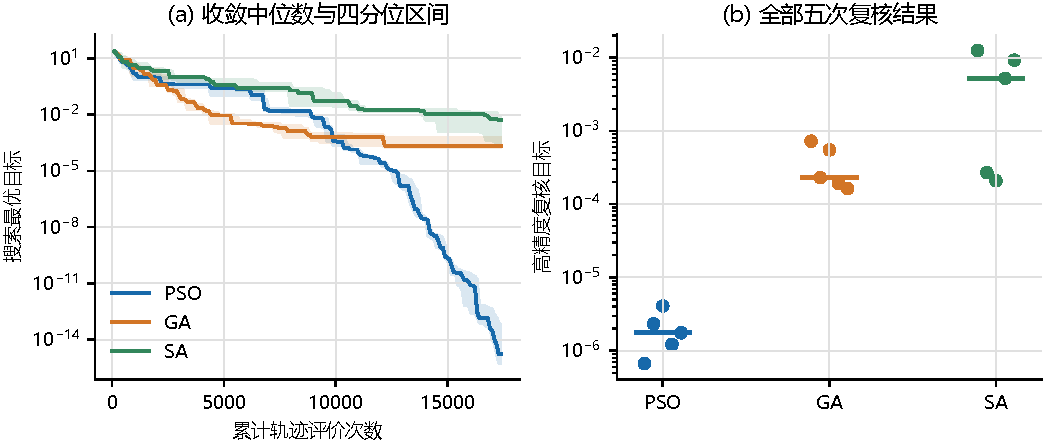
\includegraphics[width=.95\linewidth]{fig_planner_comparison.pdf}
\caption{等预算搜索与复核。左：搜索目标中位数及25\%--75\%区间；右：五个配对种子的高精度复核目标。搜索曲线与右图使用不同精度评价，不应直接等同。}\label{fig:algorithm}
\end{figure}
在当前预算与配置下，PSO的五次运行均通过高精度验收，而GA与SA的通过数均为0/5。表\ref{tab:algorithm}中，PSO的复核目标中位数低于GA和SA，说明其在本组实验中获得了更小的终端综合误差。图\ref{fig:residual}进一步显示，GA与SA虽然降低了目标值，但部分速度残差仍超过10\,m/s，成为未通过验收的主要原因。这表明归一化平方和与逐分量可行性应结合评价；单一目标值不能替代终端条件检查。
\begin{figure}[htbp]\centering
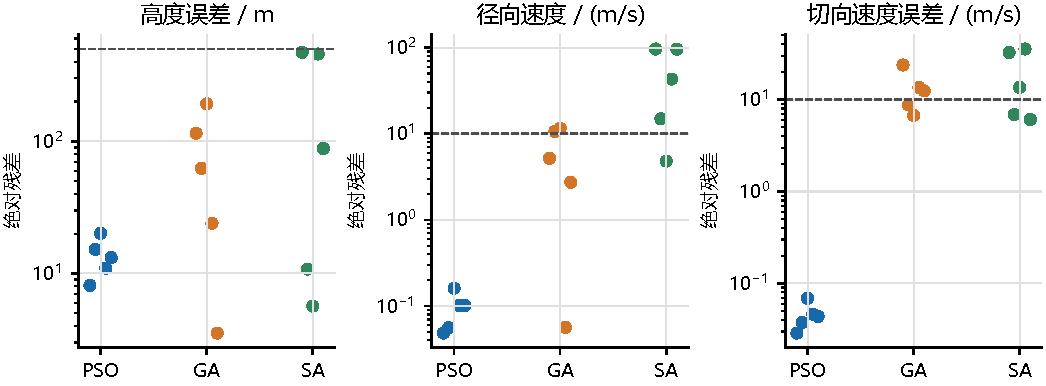
\includegraphics[width=.95\linewidth]{fig_planner_residuals.pdf}
\caption{最终候选的高精度复核残差。每点对应一次运行；虚线为高度500\,m和两速度10\,m/s验收界限。}\label{fig:residual}
\end{figure}

\subsection{搜索精度与参考轨迹}
搜索曲线与高精度复核结果之间存在明显的量级差异。PSO在定步长模型上的目标可降至极小值，而复核后的高度残差仍处于数米至数十米范围。这一差异说明，即使搜索器在离散模型上获得极小目标值，也不意味着连续动力学的终端误差同步趋近于零。因此，本文以高精度复核值作为入轨性能依据。进一步细化自适应积分后，终端径向差的最大值为\MaxFineRadius\,m，用于表征最终结果的数值敏感性。

选作MPC参考的PSO种子为\ReferenceSeed，关机时刻\ReferenceTime\,s，推进剂消耗\ReferenceFuel\,kg，高度、径向及切向速度残差分别为\ReferenceHeight\,m、\ReferenceRadial\,m/s和\ReferenceTangential\,m/s。其两段燃烧、滑行及状态演化见图\ref{fig:reference}。
\begin{figure}[htbp]\centering
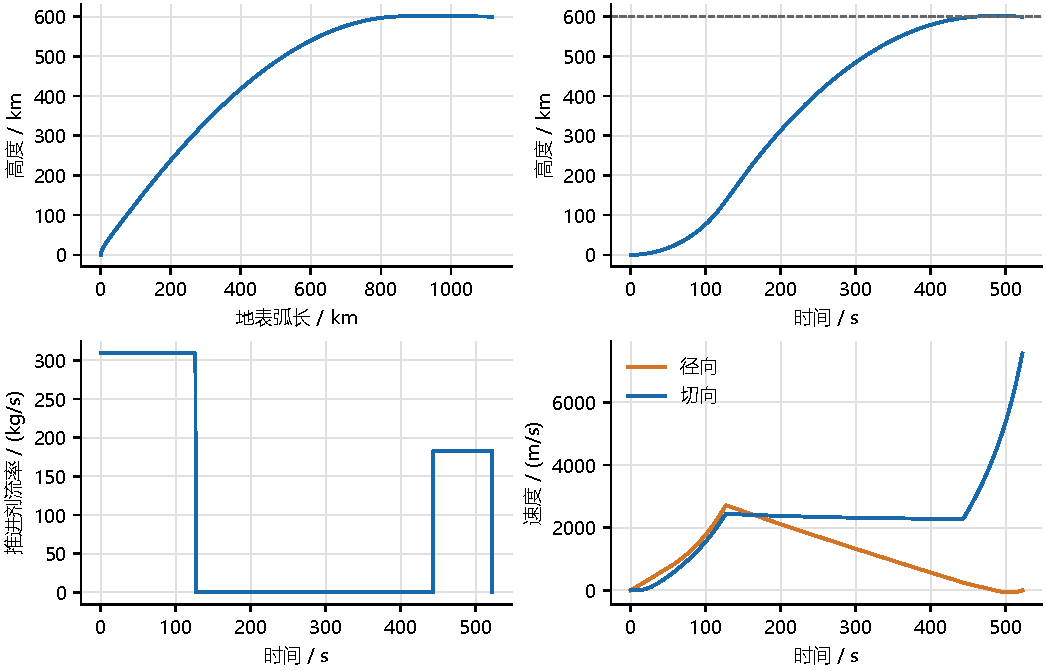
\includegraphics[width=.88\linewidth]{fig_pure_reference.pdf}
\caption{无局部精修的PSO参考：平面轨迹、高度、流率与速度时间历程。高度到达目标与速度完成圆轨化为不同要求。}\label{fig:reference}
\end{figure}
图\ref{fig:reference}展示了两段燃烧方案的阶段特征：第一段建立上升运动并积累横向速度，滑行段继续抬升高度，第二段则调节径向与切向速度以接近圆轨道条件。参考控制直接取自PSO返回参数，复核仅重新计算其动力学响应。

\subsection{独立扰动下的开闭环对照}
本组实验检验MPC对参考轨迹执行偏差的补偿作用。规划扰动种子为20261020，实际飞行采用20261021，以区分规划环境与验证环境。开环与闭环保持相同初值及实际扰动，前者执行参考前馈，后者叠加MPC反馈修正。在控制采样点上定义
\begin{equation}
E_p=\sqrt{\frac1M\sum_{j=1}^M[(r_j-\bar r_j)^2+R_E^2(\theta_j-\bar\theta_j)^2]},\quad
E_v=\sqrt{\frac1M\sum_{j=1}^M[(u_j-\bar u_j)^2+(w_j-\bar w_j)^2]} .
\end{equation}
其中，$E_p$合成径向误差与地表弧长误差，用于衡量沿参考轨迹的空间偏差。表\ref{tab:mpc}分别报告相对参考的跟踪RMS和相对目标圆轨道的关机误差，以区分轨迹执行精度与轨道注入精度。
\begin{table}[H]\centering\small
\caption{纯PSO参考的开闭环对照。}\label{tab:mpc}
\begin{tabular}{lrr}\toprule
指标 & 开环 & MPC\\\midrule
位置跟踪RMS / m & 25836.5824 & 1.9446\\
速度跟踪RMS / (m/s) & 106.6680 & 0.0976\\
关机高度误差 / m & -29848.9667 & -8.1569\\
关机径向速度 / (m/s) & -174.7328 & 0.0036\\
关机切向速度误差 / (m/s) & 101.7313 & 0.7456\\
\bottomrule\end{tabular}\end{table}
\begin{figure}[htbp]\centering
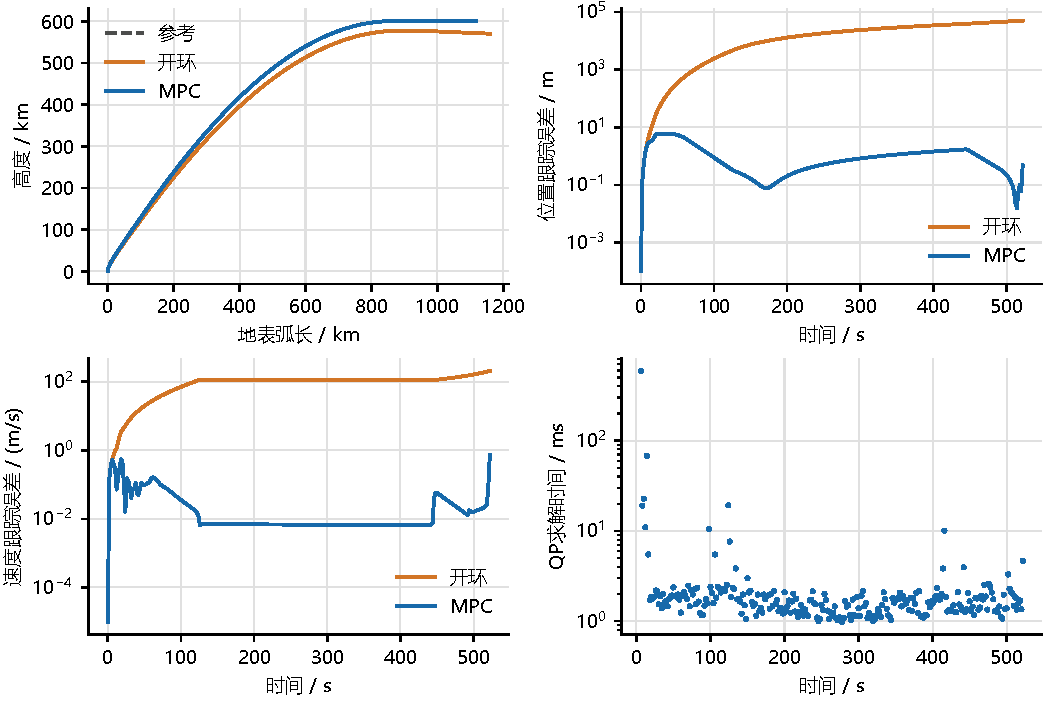
\includegraphics[width=.90\linewidth]{fig_pure_mpc.pdf}
\caption{相同实际扰动下的开环与MPC：平面轨迹、位置跟踪误差、速度跟踪误差及QP求解时间。对数误差图的零值显示下限仅用于绘图。}\label{fig:mpc}
\end{figure}
由表\ref{tab:mpc}与图\ref{fig:mpc}可见，MPC将位置跟踪RMS从开环的\OpenPos\,m降至\ClosedPos\,m，速度跟踪RMS从\OpenVel\,m/s降至\ClosedVel\,m/s。开环偏差随飞行过程积累，闭环则通过持续更新偏角与流率修正使轨迹保持在参考附近。该对照说明，性能改善来自状态反馈对执行偏差的补偿，而非初始状态或实际扰动条件的改变。参考轨迹自身仍具有非零入轨残差，因此较小的跟踪误差不意味着相对于目标轨道的误差同样为零。

在线过程中共求解\QPCount 次QP，失败\QPFail 次。单次平均耗时为\QPMean\,ms，最大耗时为\QPMax\,ms，均不包含参考线性化预计算。该结果表明，所构造的低维QP能够在本机桌面环境下完成滚动控制计算；嵌入式实现仍需结合目标硬件、测量开销和最坏情况时延进行独立评估。
